
尽管有不同的外观,大多数界面倾向于做相同的事情;因此,我们在前一节中已经介绍的大多数内容在这里也同样有效。记住,我们要改变的是互动的形式,而不是实际使用的工具。

\begin{tcolorbox}[colback=webgreen!5!white,colframe=webgreen!75!black,title=Note]
在继续之前,请检查ccmake命令在终端中是否可用。若没有,请验证您的PATH变量是否设置正确,并检查安装是否正确。
\end{tcolorbox}

\subsubsubsection{2.3.1\hspace{0.2cm}如何使用ccmake}

ccmake是CMake的一个基于终端的图形用户界面(GUI),允许用户编辑缓存的CMake变量。不叫它GUI,术语终端用户界面(TUI)可能更适合,因为没有传统的shell UI元素,如窗口和按钮。这些使用名为ncurses的文本接口框架在终端中进行呈现。

因为ccmake是默认CMake安装的一部分,所以除了CMake之外,不需要额外的安装。使用ccmake与在CLI中使用CMake完全相同,只是缺乏调用构建和安装步骤的能力。主要的区别是ccmake将显示基于终端的图形界面,用于交互式编辑缓存的CMake变量。ccmake的状态栏将显示每个设置及其可能值的描述。

开始使用ccmake,在项目配置步骤中使用ccmake。我们的例子中,将完全复制我们之前在通过CLI配置项目一节中所做的CLI示例:

\begin{tcblisting}{commandshell={}}
ccmake -G "Unix Makefiles" -S . -B ./build
\end{tcblisting}

使用示例如下所示:

\begin{center}
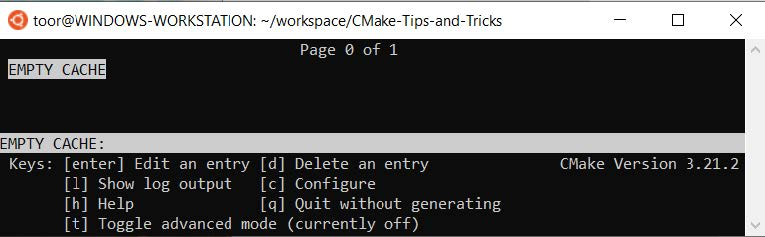
\includegraphics[width=0.8\textwidth]{content/1/chapter2/images/23.jpg}\\
图2.23 ccmake主界面
\end{center}

执行该命令后,将出现一个基于终端的用户界面。初始页面是可以编辑CMake变量的主页面,空缓存意味着没有预先配置和CMake缓存文件(CMakeCache.txt)目前是空的。为了开始编辑变量,必须首先配置项目。要进行配置,请按下键盘上的C键,如\texttt{Keys:}部分所示。

按下C键后,将执行CMake配置步骤,并进入日志输出界面,输出配置信息:

\begin{center}
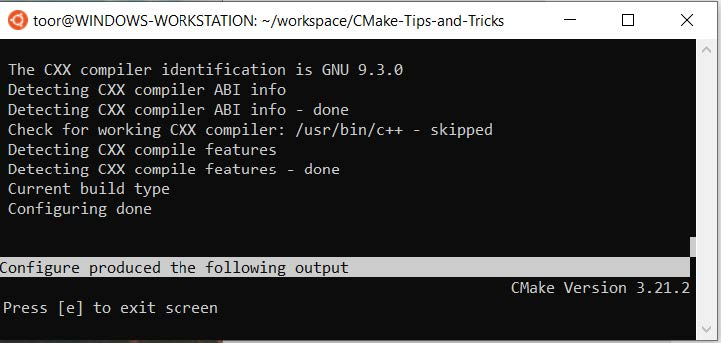
\includegraphics[width=0.8\textwidth]{content/1/chapter2/images/24.jpg}\\
图2.24 配置后ccmake的日志界面
\end{center}

关闭日志输出屏幕并返回到主屏幕,请按E。返回时,注意\texttt{EMPTY CACHE}替换成CMakeCache.txt文件中的变量名称。要选择一个变量,请使用键盘上的向上和向下箭头键。当前选中的变量将以白色高亮显示,如下图所示:

\begin{center}
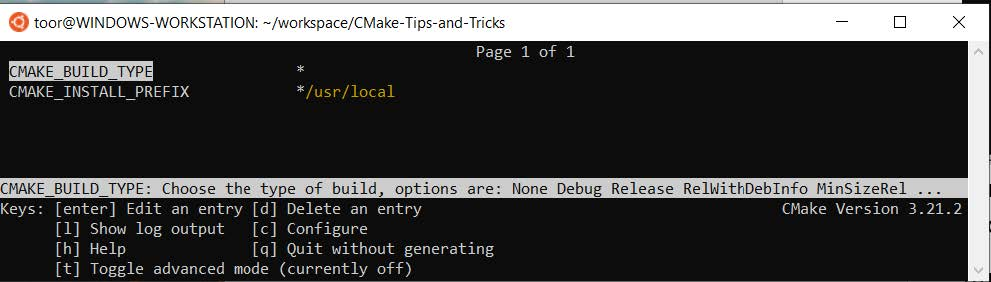
\includegraphics[width=1.\textwidth]{content/1/chapter2/images/25.jpg}\\
图2.25 配置完成后ccmake的主界面
\end{center}

前面的屏幕截图中,选择了\texttt{CMAKE\_BUILD\_TYPE}。在右边,显示了CMake变量的当前值。对于\texttt{CMAKE\_BUILD\_TYPE},现在是空的。变量值旁边的星号表示该变量的值刚刚更改了之前的配置。可以按回车键进行编辑,也可以按键盘上的D键删除。下图显示了改变变量后ccmake主界面的样子:

\begin{center}
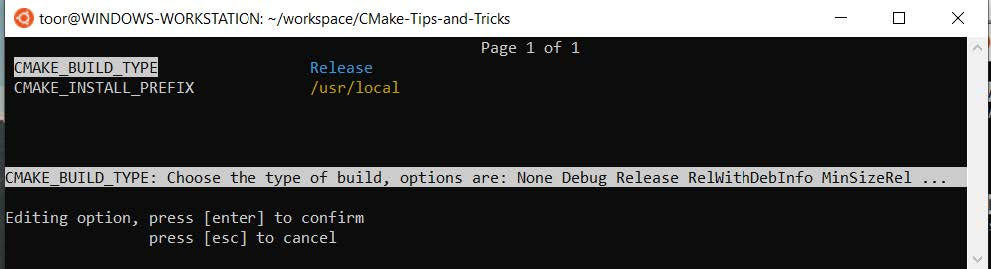
\includegraphics[width=1.\textwidth]{content/1/chapter2/images/26.jpg}\\
图2.26 ccmake的主界面随变量变化
\end{center}

让我们设置\texttt{CMAKE\_BUILD\_TYPE}为Release并再次配置:

\begin{center}
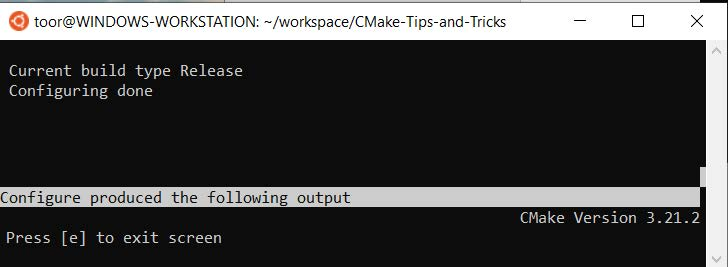
\includegraphics[width=1.\textwidth]{content/1/chapter2/images/27.jpg}\\
图2.27 ccmake配置输出(发布版)
\end{center}

可以观察到构建类型现在被设置为Release。返回到上一个屏幕,按下g(生成)按钮保存更改。可以通过按q(退出而不生成)按钮丢弃更改。

要编辑其他变量,例如:\texttt{CMAKE\_CXX\_COMPILER}和\texttt{CMAKE\_CXX\_FLAGS},高级模式应该打开。默认情况下,通过\texttt{mark\_as\_advanced()}将这些变量标记为高级变量;因此,默认情况下,它们在图形界面中是隐藏的。在主界面按“t”键可切换到高级模式。

\begin{center}
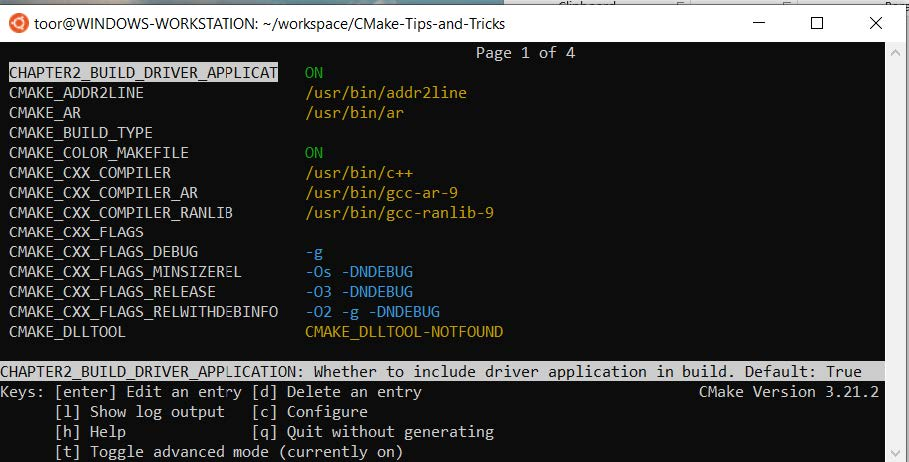
\includegraphics[width=1.\textwidth]{content/1/chapter2/images/28.jpg}\\
图2.28 - ccmake的高级模式
\end{center}

激活高级模式后,一组全新的选项将变得可见。可以观察和修改它们的值,就像普通变量一样。以前隐藏的名为\texttt{CHAPTER2\_BUILD\_DRIVER\_APPLICATION}现在出现了,这是一个用户定义的CMake变量。该变量定义如下:

\begin{lstlisting}[style=styleCMake]
# Option to exclude driver application from build.
set(CHAPTER2_BUILD_DRIVER_APPLICATION TRUE CACHE BOOL "Whether
to include driver application in build. Default: True")
# Hide this option from GUI's by default.
mark_as_advanced(CHAPTER2_BUILD_DRIVER_APPLICATION)
\end{lstlisting}

\texttt{CHAPTER2\_BUILD\_DRIVER\_APPLICATION}定义为一个布尔类型的缓存变量,默认值为true。它标记为“高级”,这就是为什么它在非高级模式中不存在的原因。

\subsubsubsection{2.3.2\hspace{0.2cm}使用cmake-gui}

若认为CLI反直觉,或者更喜欢GUI而不是CLI,那么CMake也有跨平台的GUI。与ccmake相比,cmake-gui提供了更多的功能,比如:环境编辑器和正则表达式资源管理器。

CMake GUI是默认CMake安装的一部分;除了CMake之外,不需要额外安装,主要目的是允许用户配置CMake项目。要启动cmake-gui,请在终端中发出cmake-gui命令。对于Windows,也可以从开始菜单中找到它。若这些方法都不起作用,进入CMake的安装路径,它应该在bin目录下。

\begin{tcolorbox}[colback=webgreen!5!white,colframe=webgreen!75!black,title=Note]
若在Windows环境中启动cmake-gui,并且打算使用Visual Studio提供的工具链,从IDE的适当的本地工具命令提示符启动cmake-gui。若有多个版本的IDE,请确保正在使用正确的Native Tools命令提示符。否则,CMake可能无法发现所需的工具,如编译器,或可能发现不正确的工具。更多信息请参考\url{https://docs.microsoft.com/en-us/visualstudio/ide/reference/command-prompt-powershell?view=vs-2019}。
\end{tcolorbox}

下面是CMake GUI的主窗口:

\begin{center}
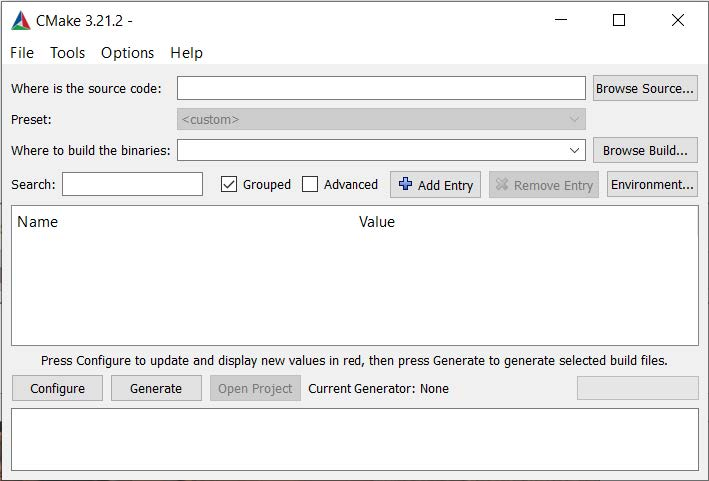
\includegraphics[width=0.6\textwidth]{content/1/chapter2/images/29.jpg}\\
图2.29 CMake GUI主窗口
\end{center}

CMake GUI的主屏幕包含以下内容:

\begin{itemize}
\item 
源代码路径字段

\item 
输出路径字段

\item 
配置和生成按钮

\item 
缓存变量列表
\end{itemize}

这是我们将要与之互动的四件重要的事情。要开始配置项目,请单击\texttt{Browse Source…}按钮,选择项目的根目录,通过单击\texttt{Browse Build…}按钮为项目选择一个输出目录。此路径将是所选生成器生成的输出文件的路径。

设置源和输出路径后,单击\texttt{Configure}开始配置所选项目。CMake GUI可以让你选择使用的生成器、平台选择(如果生成器支持的话)、工具集和编译器等细节,如下图所示:

\begin{center}
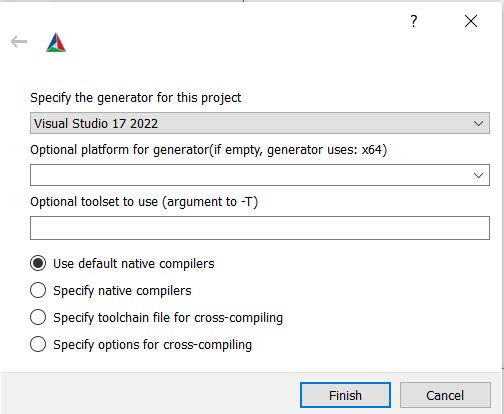
\includegraphics[width=0.6\textwidth]{content/1/chapter2/images/30.jpg}\\
图2.30 CMake GUI生成器选择窗口
\end{center}

根据环境填写这些详细信息之后,单击\texttt{Finish}继续。CMake GUI将开始使用给定的详细信息配置您的项目,并在日志部分报告输出。配置成功后,也应该在缓存变量列表部分看到缓存变量:

\begin{center}
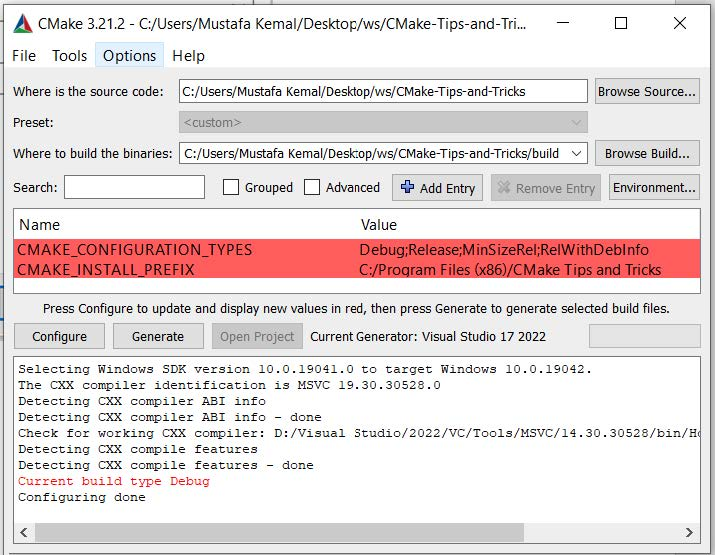
\includegraphics[width=0.8\textwidth]{content/1/chapter2/images/31.jpg}\\
图2.31 配置后的CMake GUI
\end{center}

若一切正常,请按\texttt{Generate}按钮生成所选构建系统所需的构建文件。对于Visual Studio生成器,生成的文件是.sln和.cxxproj以及其他文件。在生成项目之后,\texttt{Open project}按钮将启用,可用其使用适当的编辑器或IDE打开生成的项目。若构建系统没有与任何IDE关联(例如,makefiles),那么生成的文件将显示出来,并可以使用IDE构建项目。

\begin{tcolorbox}[colback=webgreen!5!white,colframe=webgreen!75!black,title=重要Note]
生成的项目只是生成器的工件,对生成的项目文件的更改(.sln, .cxxproj)将不会被保存,并将在下次生成中丢失。当修改CMakeLists.txt文件或编辑CMakeCache.txt文件时,不要忘记重新生成项目文件(直接或间接)。对于版本控制方面,应该将生成的项目文件视为构建工件,而不该将它们添加到版本控制中。可以通过CMake和合适的生成器生成项目来重新生成。
\end{tcolorbox}

有时,项目可能需要调整一些缓存变量,或者需要决定使用不同的构建类型。要更改任何缓存变量,请单击所需缓存变量的值;应该可以编辑。根据变量类型的不同,可能会显示复选框而不是字符串。若所需的变量在列表中不可见,则可能是高级变量,只有选中窗口上的\texttt{advanced}复选框时才可见。还可以使用搜索框更容易地定位变量,还可以在\texttt{cmake-gui}的高级模式下看到:

\begin{center}
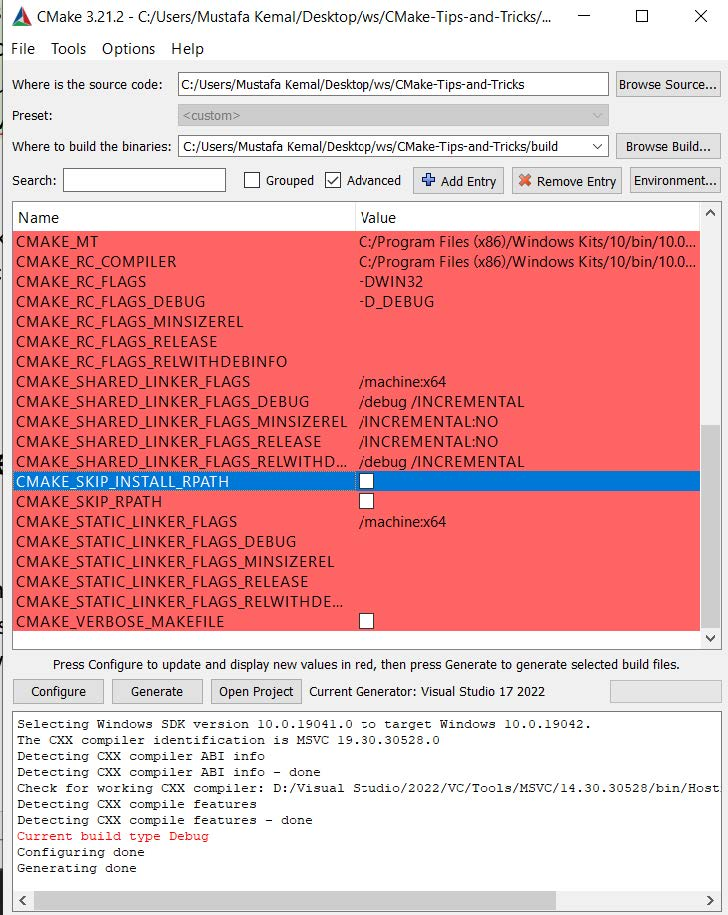
\includegraphics[width=0.6\textwidth]{content/1/chapter2/images/32.jpg}\\
图2.32 高级模式下的cmake-gui
\end{center}

调整缓存值之后,单击\texttt{Configure},然后单击\texttt{Generate}应用更改。

\begin{tcolorbox}[colback=webgreen!5!white,colframe=webgreen!75!black,title=Tip]
另一个特性是分组特性,可以将缓存变量分组到公共前缀中(有的话)。组名由变量名的第一部分确定,直到第一个下划线为止。
\end{tcolorbox}

已经介绍了cmake-gui的最基本特性。在处理其他杂项之前,若需要重新加载缓存值或删除缓存并从头开始,可以在文件菜单中找到“Reload Cache”和“Delete Cache”菜单项。

\subsubsubsection{2.3.3\hspace{0.2cm}修改环境变量}

CMake GUI提供了一个方便的环境变量编辑器,允许对环境变量进行CRUD操作。要访问它,只需单击主屏幕上的\texttt{Environment…}按钮。点击后,会弹出“Environment Editor”窗口,如下图所示:

\begin{center}
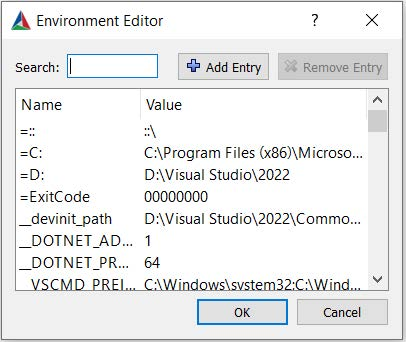
\includegraphics[width=0.6\textwidth]{content/1/chapter2/images/33.jpg}\\
图2.33  CMake GUI环境变量编辑器
\end{center}

Environment Editor窗口包含当前环境中存在的环境变量列表。要编辑环境变量,双击表中所需环境变量的值字段。该窗口还允许通过添加条目和删除条目按钮添加和删除信息。

\subsubsubsection{2.3.4\hspace{0.2cm}对正则表达式求值}

有没有想过一个正则表达式,会如何得到CMake的评估,以及会给出什么结果?若有这样的想法,您可能已经通过\texttt{message()}打印了regex匹配结果的变量。若有更好的方法呢?这里来看下CMake GUI的正则表达式资源管理器工具。

\begin{center}
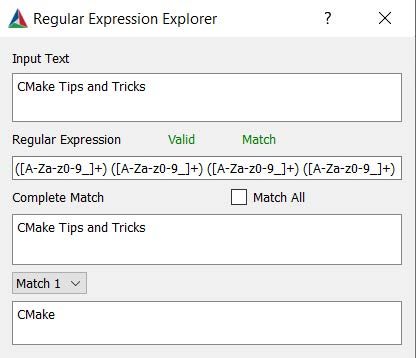
\includegraphics[width=0.6\textwidth]{content/1/chapter2/images/34.jpg}\\
图2.34  CMake GUI正则表达式资源管理器
\end{center}

这个隐藏的gem允许使用CMake的regex引擎调试正则表达式它位于“工具”菜单中,名称为\texttt{Regular Expressions Explorer…},使用起来非常简单:

\begin{enumerate}
\item 
在正则表达式字段中输入表达式。

该工具将检查表达式是否有效。若有效,屏幕上的有效文本将是绿色的。如果CMake的regex引擎不喜欢你给出的表达式,它会变成红色。

\item 
在\texttt{Input Text}字段中输入测试字符串。正则表达式将与此文本匹配。

\item 
若有任何匹配,窗口上的\texttt{match}将从红色变为绿色。匹配的字符串将在完全匹配字段中打印出来。

\item 
匹配时,捕获组将被分配给匹配1、匹配2和匹配N(有的话)。
\end{enumerate}

本节中,我们学习了如何使用CMake的本机图形界面。接下来,通过了解CMake的IDE和编辑器集成来继续学习CMake的使用。
